%!TEX root = ../thesis.tex
%*******************************************************************************
%****************************** Second Chapter *********************************
%*******************************************************************************

\chapter{State-of-the-Art}

\ifpdf
    \graphicspath{{Chapter2/Figs/Raster/}{Chapter2/Figs/PDF/}{Chapter2/Figs/}}
\else
    \graphicspath{{Chapter2/Figs/Vector/}{Chapter2/Figs/}}
\fi

\textbf{Wikification} its an automatic process inspired by \textit{Wikipedians}\footnote{\textit{Wikipedian}, also known as editor, is a contributor from the Wikipedia Community, who volunteers to write and edit Wikipedia's articles. 
Anyone who edit or find something that can be improved in the Wikipedia articles can become a Wikipedian.}
Wikipedians manually select words or phrases that are considered relevant in an article and link it to another Wikipedia article which title are closely related to this words and phrases.

According to \citep{Mihalcea2007} \textbf{Wikification} is ``\textit{the automatically extraction of words or terms that are the most importants in a document and for each of this keywords in an article identify the most appropiate article in
Wikipedia}''.

For humans this in an easy process, but it is a hardly process to get it done automatically \citep{Roris2014}.
A Wikipedian links articles from Wikipedia according to the knowledge he or she has from a topic, that is a tasks done by her or his personal apreciation about a concept they consider must be explain.

\dots and some more

In this chapter we will provide an overview of some relevant approaches related to Wikification Process

\section[Relevant approaches related to Wikification Process]{Relevant approaches related to Wikification Process}

% Uncomment this line, when you have siunitx package loaded.
%The SI Units for dynamic viscosity is \si{\newton\second\per\metre\squared}.
%I'm going to randomly include a picture Figure~\ref{fig:minion}.


%If you have trouble viewing this document contact Krishna at: \href{mailto:kks32@cam.ac.uk}{kks32@cam.ac.uk} or raise an issue at \url{https://github.com/kks32/phd-thesis-template/}
This work is related to the next natural language processing issues:

\section*{Itemize}
\begin{itemize}
\item Word sense desambiguation problem
\item Machine learning problem
\item Keyword extraction
\item Document and text processing
\end{itemize}

Some approaches have been proposed with big influence in the selection and methodology used for the Wikification process
about to be describe in the next sections.

Wikipedia has become a very large and rich source of information and is the input for the next related work.

\subsubsection{Wikipedia as a Dataset}
One thing that must be considered when working with Wikipedia data, is dealing with her size, specially the English-language 
edition\footnote{Size of Wikipedia, \url{https://en.wikipedia.org/wiki/Wikipedia:Size_of_Wikipedia}} 
with approximately 5,360,487 articles on the site (live count) is the biggest one with the most articles of any of the other Wikipedias.
In October 2015, the combined text of the English Wikipedia's articles totalled 11.5 gigabytes when compressed and  on November 1st 2015, 
the English Wikipedia announced it had reached 5,000,000 articles and ran a special logo to reflect the milestone.

\begin{figure}[htbp!] 
\centering    
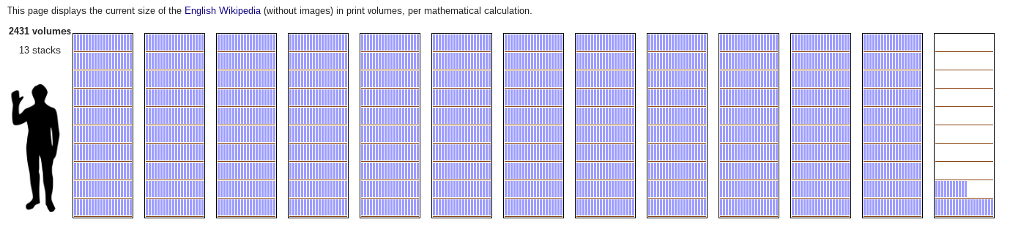
\includegraphics[width=1.0\textwidth]{EWinVolumnes}
\caption[EWinVolumnes]{Representation of the current size of the English Wikipedia (without images) in print volumes, per mathematical calculation. \url{https://en.wikipedia.org/wiki/Wikipedia:Size_in_volumes}}
\label{fig:EWinVolumnes}
\end{figure}
%------------------------
\subsection{David Milne and Ian H. Witten - Learning to link with Wikipedia}

cross-reference documents with Wikipedia by identifying significant terms within unstructured text using machine learning and enrich it with links to the appropriate Wikipedia articles.

They describe their work as a link detector and disambiguator, able to enrich any unstructured fragment of text which is automatically recognized and linked with structured knowledge, in this case with Wikipedia articles.

The uses machine-learning approach to disambiguate links for the wikification process.

For the experiments Milne and Witten, worked with a Wikipedia snapshot from November 20, 2007 that contained under two million articles. 
They selected articles containing at least 50 links, avoided list and disambiguation pages because they were considered not representative unstructured text. 

A total of 700 articles were randomly selected and set aside for developing the disambiguation algorithm: 500 were used for training, 100 for configuration, and a further 100 for final
evaluation.

The 500 training articles contain more than 50,000 links. Each link represents several training instances, they built an anchor tree with the possible senses, 
only one sense is a positive example and the rest are negative. As explained before, an anchor are phrases that link to a target.

They used the same approach than Mendelyan et al. to balance the commonness of a sense with its relatedness to the sorrounding text. 
The commonness or prior probability is computed by the number of times it is used as a destination in Wikipedia, but they compare each possible sense 
with its sorrounding context and also use every unambiguous link in the document as context to the disambiguation process. 
Each candidate sense and context term is represented by a single Wikipedia article, so they solve selecting the sense article that has most in 
common when comparing with all of the context articles, the relatedness. 

They used a method they also already developed \citep{AAAI:2008:milne} to measure the semantic similarity of two Wikipedia pages 
known as Wikipedia Link-based Measure, which compares the incoming and outgoing links, expressed in the next formula:

\begin{equation}
relatedness \left( a, b \right) = \frac{\log \left( \max \left( \left| A \right|, \left| B \right| \right) \right) - \log \left( \left| A \cap B \right| \right)}
                                       {\log \left( \left| W \right| \right) - \log \left( \min \left( \left| A \right|, \left| B \right| \right) \right)}
\end{equation}

Where {\em a} and {\em b} are two articles, {\em A} and {\em B} are sets of all the articles that link to {\em a} and link to {\em b} and {\em W} is the set of all the articles in Wikipedia.

As mentioned before the approach use the information from the context to determine how closely related to the central thread the terms are, 
and is determine by two main features (1) link probability proposed by Mihalcea and Csomai that provides the commonness of each sense and (2) semantic relatedness. 
A third feature is involve —the context quality—which ss given by the sum of the weights that were previously assigned to each context term. 
This three features are used to train the classifier. A diference from other approaches in the desambioguation process is that Milne and Witten can be done in two ways:

\begin{enumerate}
 \item considering each sense independently with an assigned probability, this implies that it could be not the best sense but a valid one.
 \item using the sense with the highest probability or the set of senses that may be useful, and with the higher probability of being valid than not.
\end{enumerate}

%------------------------
\subsection{Rada Mihalcea and Andras Csomai - Wikify! Linking Documents to Encyclopedic knowledge}

The autors assert that Wikipedia \url{http://en.wikipedia.org} can be used to achive state-of-the-art results on both,
1) keyword extraction and 2) word sense disambiguation.

The Wikify! system was designed and implemented with two visions: 

\begin{enumerate}
 \item Semantic Web, it could be used for automatically enrich online documents with references to semantically related information,
 \item As a tool that could be used for education porpouses, capable to link important terms to encyclopedic pages as a gateway between for example lecture notes, 
       teaching materials, assigments.
\end{enumerate}

For the experiments Mihalcea and Csomai, worked with a Wikipedia download from March 2006, with approximately 1.4 million articles and more
then 37 millions hyperlinks.

\subsubsection{Text Wikification}
The first task \textbf{keyword extraction} is about the identification of those words and relevant phrases 
that best describe the subject of a document \footnote{Keyword extraction, \url{https://en.wikipedia.org/wiki/Keyword_extraction}}.


The second task \textbf{link a candidate keyword with the correct Wikipedia article}, for what word sense disambiguation
must be perform and context is taken in consideration and the {\em disambiguation pages} play an important rol in the process.

Some of the decisions taken for this task were supported by the Wikipedia manual of style, like 1) selecting links to provide deeper
understanding of the topic or particular terms, such as technical terms, names, places that means only links relevant to the context
\footnote{Wikipedia:Manual of Style/Linking, \url{https://en.wikipedia.org/wiki/Wikipedia:Manual_of_Style/Linking}},
2) Avoid terms unrelated to the main topic, 3) Proper amount of keywords in an article, too many links could obstruct the reading.

They aware the similarity  between this recommendations and the keyword extraction problem, so they address the solution as
a keyword extraction task, the recommendations derived in decisions for the system, like constructing controlled vocabulary with
1,918,830 terms including the Wikipedia article titles and extended to include morphological variations taking in consideration
all the surface forms collected from all the Wikipedia articles and discounting all the ocurrences that were used less than
five times.

The controlled vocabulary included acceptable phrases, the next steps deal with {\em candidate extraction} in the input document, 
which is done taking all possible n-grams that are also present in the controlled vocabulary and {\em ranking keywords} 
for reflecting the likelihood given to a keyphrase, they used:

\begin{itemize}
 \item {\em tf.idf}
 \item $x^2$ {\em independence test}       
 \item {\em keyphraseness}
\end{itemize}



\section*{Enumeration}
Lorem ipsum dolor sit amet, consectetur adipiscing elit. Sed vitae laoreet lectus. Donec lacus quam, malesuada ut erat vel, consectetur eleifend tellus. Aliquam non feugiat lacus. Interdum et malesuada fames ac ante ipsum primis in faucibus. Quisque a dolor sit amet dui malesuada malesuada id ac metus. Phasellus posuere egestas mauris, sed porta arcu vulputate ut. Donec arcu erat, ultrices et nisl ut, ultricies facilisis urna. Quisque iaculis, lorem non maximus pretium, dui eros auctor quam, sed sodales libero felis vel orci. Aliquam neque nunc, elementum id accumsan eu, varius eu enim. Aliquam blandit ante et ligula tempor pharetra. Donec molestie porttitor commodo. Integer rutrum turpis ac erat tristique cursus. Sed venenatis urna vel tempus venenatis. Nam eu rhoncus eros, et condimentum elit. Quisque risus turpis, aliquam eget euismod id, gravida in odio. Nunc elementum nibh risus, ut faucibus mauris molestie eu.
 Vivamus quis nunc nec nisl vulputate fringilla. Duis tempus libero ac justo laoreet tincidunt. Fusce sagittis gravida magna, pharetra venenatis mauris semper at. Nullam eleifend felis a elementum sagittis. In vel turpis eu metus euismod tempus eget sit amet tortor. Donec eu rhoncus libero, quis iaculis lectus. Aliquam erat volutpat. Proin id ullamcorper tortor. Fusce vestibulum a enim non volutpat. Nam ut interdum nulla. Proin lacinia felis malesuada arcu aliquet fringilla. Aliquam condimentum, tellus eget maximus porttitor, quam sem luctus massa, eu fermentum arcu diam ac massa. Praesent ut quam id leo molestie rhoncus. Praesent nec odio eget turpis bibendum eleifend non sit amet mi. Curabitur placerat finibus velit, eu ultricies risus imperdiet ut. Suspendisse lorem orci, luctus porta eros a, commodo maximus nisi.

Nunc et dolor diam. Phasellus eu justo vitae diam vehicula tristique. Vestibulum vulputate cursus turpis nec commodo. Etiam elementum sit amet erat et pellentesque. In eu augue sed tortor mollis tincidunt. Mauris eros dui, sagittis vestibulum vestibulum vitae, molestie a velit. Donec non felis ut velit aliquam convallis sit amet sit amet velit. Aliquam vulputate, elit in lacinia lacinia, odio lacus consectetur quam, sit amet facilisis mi justo id magna. Curabitur aliquet pulvinar eros. Cras metus enim, tristique ut magna a, interdum egestas nibh. Aenean lorem odio, varius a sollicitudin non, cursus a odio. Vestibulum ante ipsum primis in faucibus orci luctus et ultrices posuere cubilia Curae; 
\begin{enumerate}
\item The first topic is dull
\item The second topic is duller
\begin{enumerate}
\item The first subtopic is silly
\item The second subtopic is stupid
\end{enumerate}
\item The third topic is the dullest
\end{enumerate}
Morbi bibendum est aliquam, hendrerit dolor ac, pretium sem. Nunc molestie, dui in euismod finibus, nunc enim viverra enim, eu mattis mi metus id libero. Cras sed accumsan justo, ut volutpat ipsum. Nam faucibus auctor molestie. Morbi sit amet eros a justo pretium aliquet. Maecenas tempor risus sit amet tincidunt tincidunt. Curabitur dapibus gravida gravida. Vivamus porta ullamcorper nisi eu molestie. Ut pretium nisl eu facilisis tempor. Nulla rutrum tincidunt justo, id placerat lacus laoreet et. Sed cursus lobortis vehicula. Donec sed tortor et est cursus pellentesque sit amet sed velit. Proin efficitur posuere felis, porta auctor nunc. Etiam non porta risus. Pellentesque lacinia eros at ante iaculis, sed aliquet ipsum volutpat. Suspendisse potenti.

Ut ultrices lectus sed sagittis varius. Nulla facilisi. Nullam tortor sem, placerat nec condimentum eu, tristique eget ex. Nullam pretium tellus ut nibh accumsan elementum. Aliquam posuere gravida tellus, id imperdiet nulla rutrum imperdiet. Nulla pretium ullamcorper quam, non iaculis orci consectetur eget. Curabitur non laoreet nisl. Maecenas lacinia, lorem vel tincidunt cursus, odio lorem aliquet est, gravida auctor arcu urna id enim. Morbi accumsan bibendum ipsum, ut maximus dui placerat vitae. Nullam pretium ac tortor nec venenatis. Nunc non aliquet neque. 



\section*{Description}
\begin{description}
\item[The first topic] is dull
\item[The second topic] is duller
\begin{description}
\item[The first subtopic] is silly
\item[The second subtopic] is stupid
\end{description}
\item[The third topic] is the dullest
\end{description}


\clearpage

\tochide\section{Hidden section}
\textbf{Lorem ipsum dolor sit amet}, \textit{consectetur adipiscing elit}. In magna nisi, aliquam id blandit id, congue ac est. Fusce porta consequat leo. Proin feugiat at felis vel consectetur. Ut tempus ipsum sit amet congue posuere. Nulla varius rutrum quam. Donec sed purus luctus, faucibus velit id, ultrices sapien. Cras diam purus, tincidunt eget tristique ut, egestas quis nulla. Curabitur vel iaculis lectus. Nunc nulla urna, ultrices et eleifend in, accumsan ut erat. In ut ante leo. Aenean a lacinia nisl, sit amet ullamcorper dolor. Maecenas blandit, tortor ut scelerisque congue, velit diam volutpat metus, sed vestibulum eros justo ut nulla. Etiam nec ipsum non enim luctus porta in in massa. Cras arcu urna, malesuada ut tellus ut, pellentesque mollis risus.Morbi vel tortor imperdiet arcu auctor mattis sit amet eu nisi. Nulla gravida urna vel nisl egestas varius. Aliquam posuere ante quis malesuada dignissim. Mauris ultrices tristique eros, a dignissim nisl iaculis nec. Praesent dapibus tincidunt mauris 
nec tempor. Curabitur et consequat nisi. Quisque viverra egestas risus, ut sodales enim blandit at. Mauris quis odio nulla. Cras euismod turpis magna, in facilisis diam congue non. Mauris faucibus nisl a orci dictum, et tempus mi cursus.

Etiam elementum tristique lacus, sit amet eleifend nibh eleifend sed \footnote{My footnote goes blah blah blah! \dots}. Maecenas dapibu augue ut urna malesuada, non tempor nibh mollis. Donec sed sem sollicitudin, convallis velit aliquam, tincidunt diam. In eu venenatis lorem. Aliquam non augue porttitor tellus faucibus porta et nec ante. Proin sodales, libero vitae commodo sodales, dolor nisi cursus magna, non tincidunt ipsum nibh eget purus. Nam rutrum tincidunt arcu, tincidunt vulputate mi sagittis id. Proin et nisi nec orci tincidunt auctor et porta elit. Praesent eu dolor ac magna cursus euismod. Integer non dictum nunc.


\begin{landscape}

\section*{Subplots}
I can cite Wall-E (see Fig.~\ref{fig:WallE}) and Minions in despicable me (Fig.~\ref{fig:Minnion}) or I can cite the whole figure as Fig.~\ref{fig:animations}


\begin{figure}
  \centering
  \begin{subfigure}[b]{0.3\textwidth}
    
\includegraphics[width=\textwidth]{TomandJerry}
    \caption{Tom and Jerry}
    \label{fig:TomJerry}   
  \end{subfigure}             
  \begin{subfigure}[b]{0.3\textwidth}
    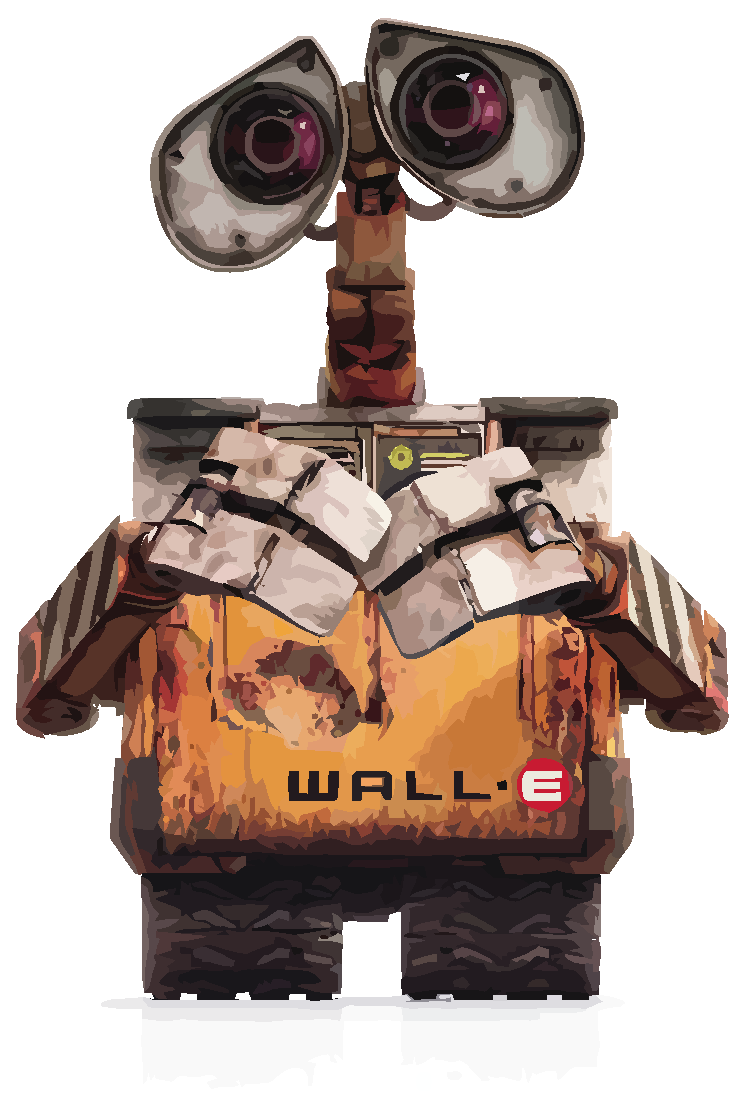
\includegraphics[width=\textwidth]{WallE}
    \caption{Wall-E}
    \label{fig:WallE}
  \end{subfigure}             
  \begin{subfigure}[b]{0.3\textwidth}
    
\includegraphics[width=\textwidth]{minion}
    \caption{Minions}
    \label{fig:Minnion}
  \end{subfigure}
  \caption{Best Animations}
  \label{fig:animations}
\end{figure}


\end{landscape}
